\header{
    \section{La blanche hermine} \label{la-blanche-hermine}
    %
    \insertComment{Chanson de Gilles Servat (1971).}{L'hermine est l'animal emblématique du duché de Bretagne.}
}

\enluminure{3}{\href{https://www.youtube.com/watch?v=X-vIVwPRtf8}{J}}{'ai} rencontré ce matin devant la haie de mon champ
\\Une troupe de marins d'ouvriers de paysans
\\Où allez-vous camarades avec vos fusils chargés
\\Nous tendrons des embuscades viens rejoindre notre armée
\\\\\textbf{Refrain :}
\\La voilà la Blanche Hermine vive la mouette et l'ajonc
\\La voilà la Blanche Hermine vive Fougères et Clisson!
\\\\Où allez-vous camarades avec vos fusils chargés
\\Nous tendrons des embuscades viens rejoindre notre armée
\\Ma mie dit que c'est folie d'aller faire la guerre aux Francs
\\Mais je dis que c'est folie d'être enchaîné plus longtemps
\\\\Elle me dit que c'est folie d'aller faire la guerre aux Francs
\\Mais je dis que c'est folie d'être enchaîné plus longtemps
\\Elle aura bien de la peine pour élever les enfants
\\Elle aura bien de la peine car je m'en vais pour longtemps
\\\\Elle aura bien de la peine pour élever les enfants
\\Elle aura bien de la peine car je m'en vais pour longtemps
\\Je viendrai à la nuit noire tant que la guerre durera
\\Comme les femmes en noir triste et seule elle m'attendra
\\\\Je viendrai à la nuit noire tant que la guerre durera
\\Comme les femmes en noir triste et seule elle m'attendra
\\Et sans doute pense-t-elle que je suis en déraison
\\De la voir mon coeur se serre là-bas devant la maison
\\\\Et sans doute pense-t-elle que je suis en déraison
\\De la voir mon coeur se serre là-bas devant la maison
\\Et si je meurs à la guerre pourra-t-elle me pardonner
\\D'avoir préféré ma terre à l'amour qu'elle me donnait
\\\\Et si je meurs à la guerre pourra-t-elle me pardonner
\\D'avoir préféré ma terre à l'amour qu'elle me donnait
\\J'ai rencontré ce matin devant la haie de mon champ
\\Une troupe de marins, d'ouvriers, de paysans
\\\\
\bigskip
\begin{center}
   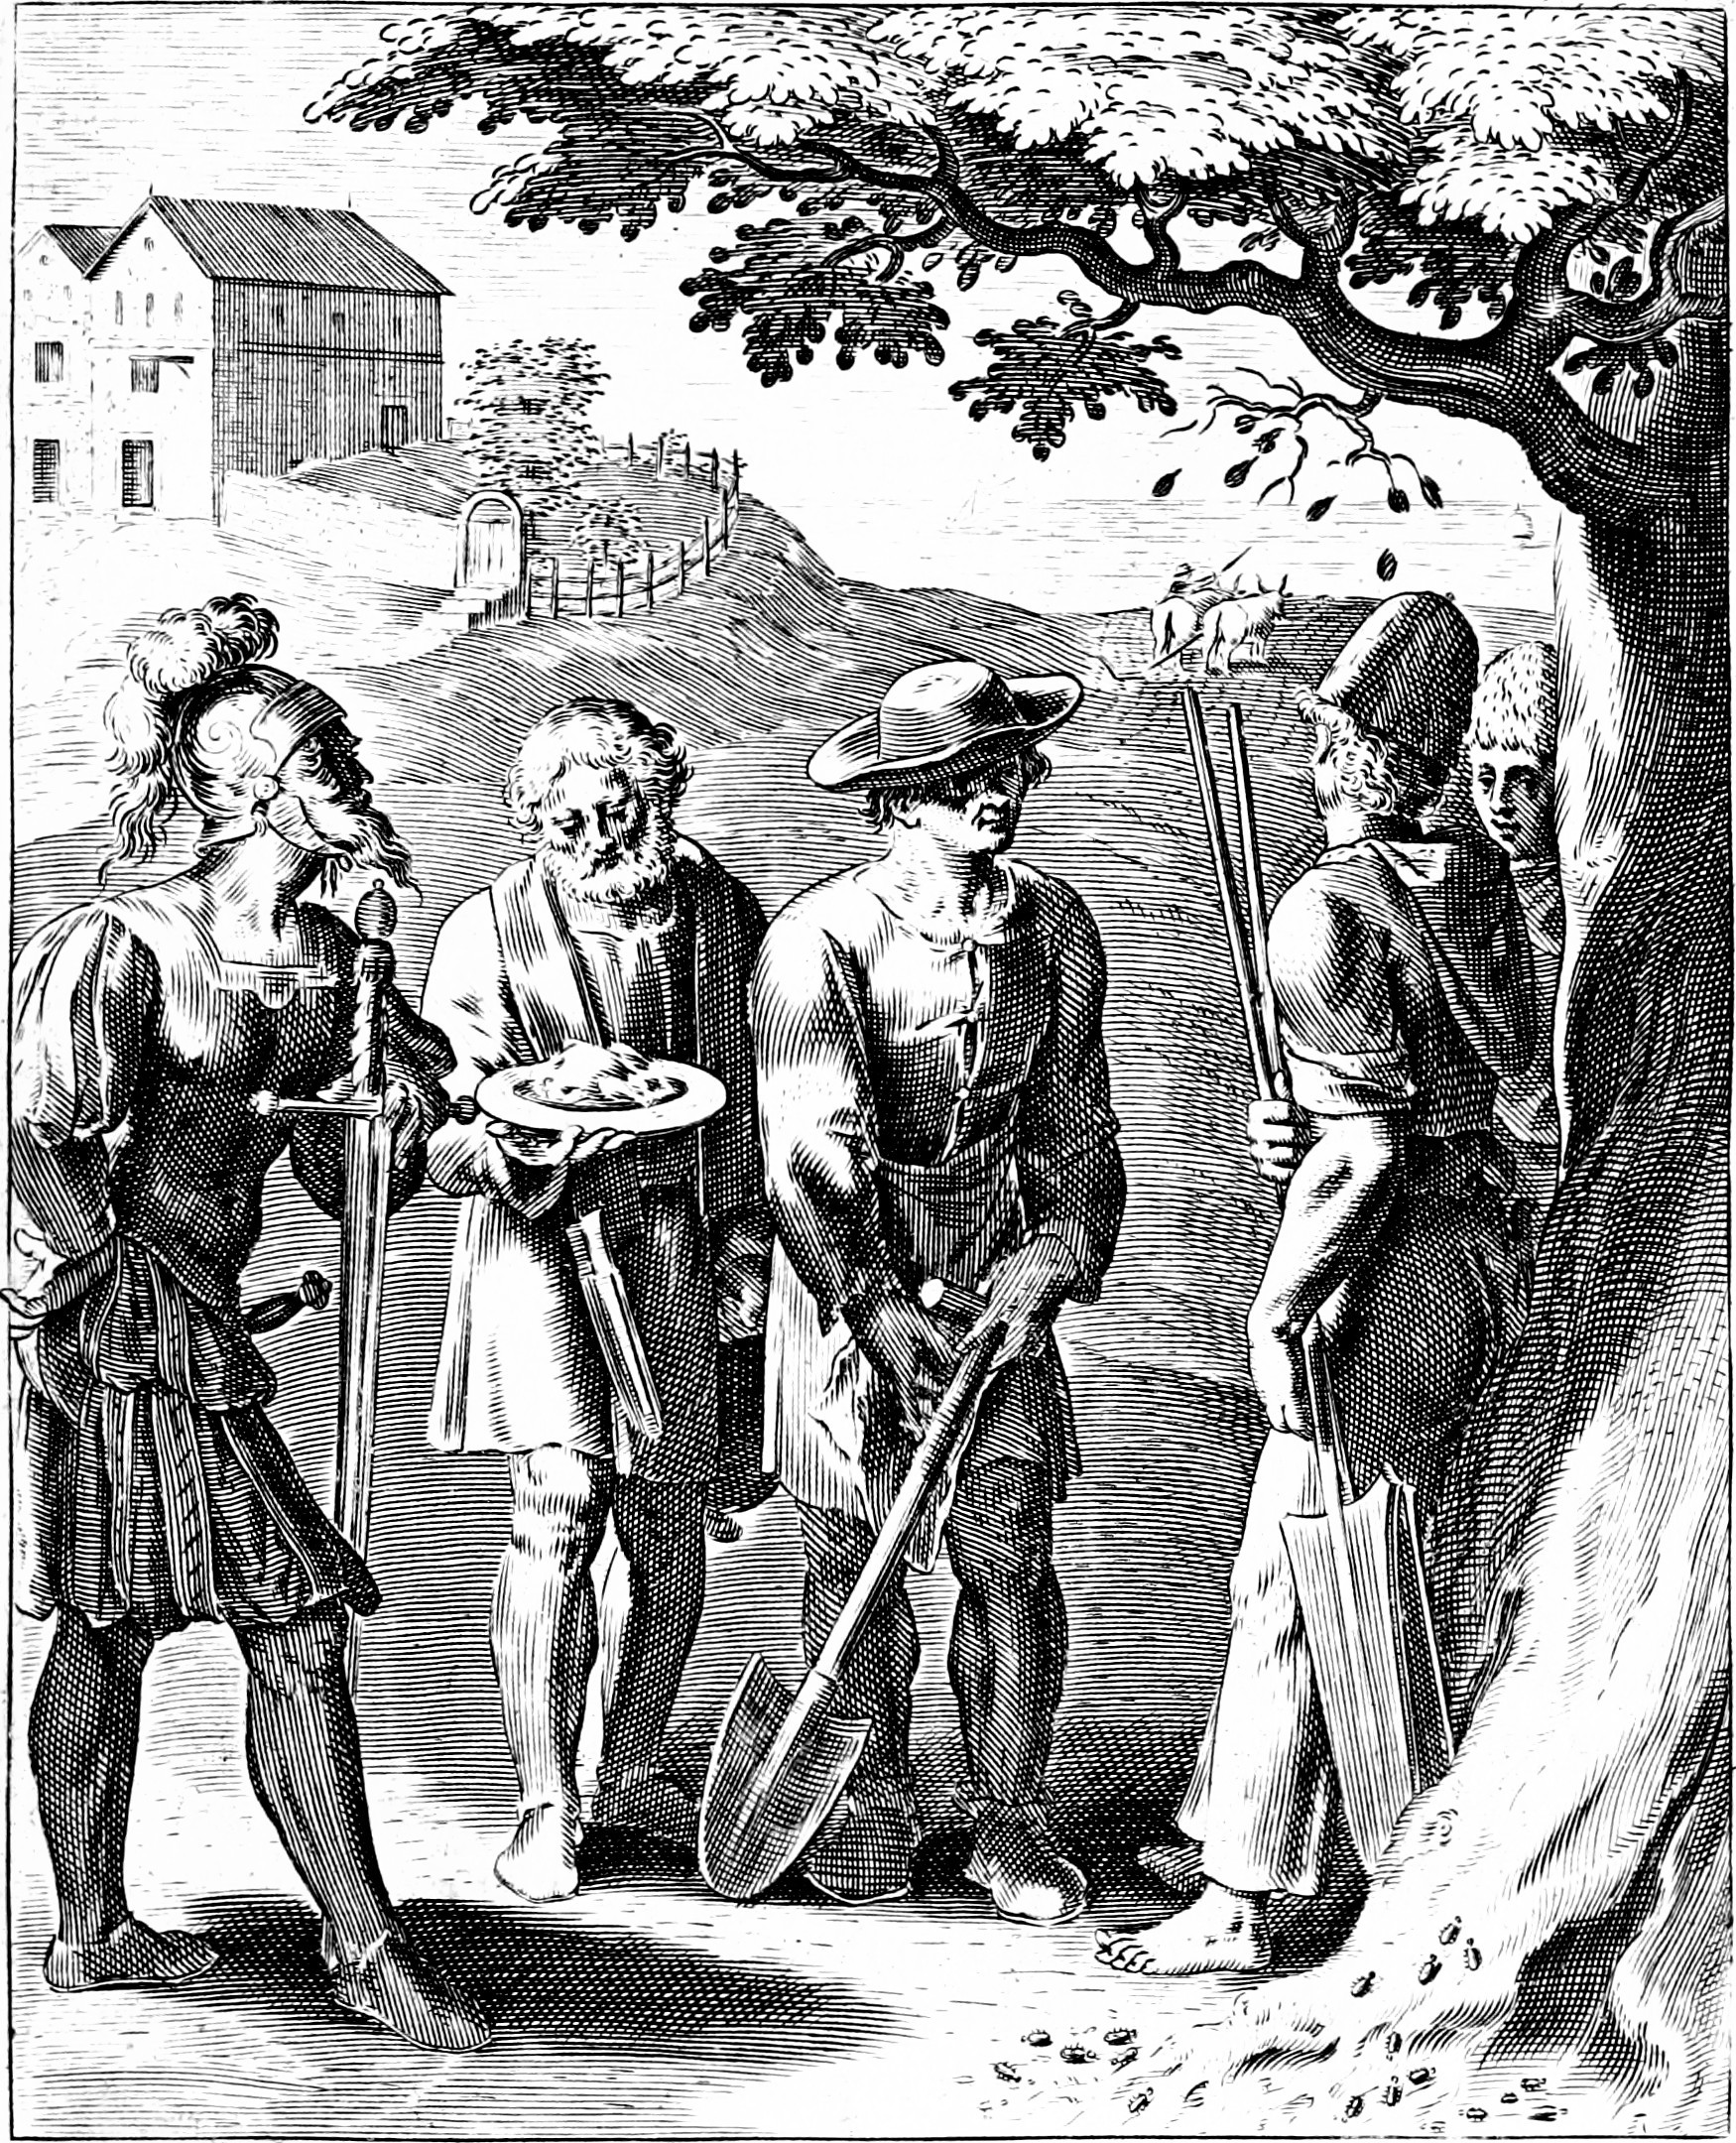
\includegraphics[width=1\textwidth]{images/brev22.png}
 \end{center}

\breakpage